\documentclass[UTF8]{ctexart}
	\title{Matrix题解}
	\author{唐适之}
	\date{}
	\newcommand{\myparagraph}[1]{\paragraph{#1}\mbox{}\\}
	\usepackage[top=1in, bottom=1in, left=1.25in, right=1.25in]{geometry}
	\usepackage{graphicx}

\begin{document}
	
	\maketitle
	
		本题考察的是通过构造解题,虽可以用数据结构进一步优化,但不作要求。
	
	\myparagraph{算法1}
		
		$O(n!)$暴力枚举所有可能的排列,$O(n^2)$扫描判断每一行是否合法。时间复杂度$O(n!n^2)$,空间复杂度$O(n^2)$,期望得分20分。
		
	\myparagraph{算法2}
	
		将直接枚举排列改成压位的记忆化搜索。仍然是搜索列的排列。记我们现在已经确定了矩阵b的前x列,这x列对应原矩阵a的y这些列,y是一个用二进制表示的列集合。对于第r行,如果前x列包含其所有1或全部为0,那么前x列的具体排列对后n-x列无影响;否则,那么第r行第x列必须是1,除此之外后n-x列依然与前x列的具体排列无关。所以对于每一个二元组(x,y)只用搜索一遍。(x,y)共有$2^n$种,除此之外,对于每个(x,y)我们还需要使用$O(n^2)$的时间枚举第x+1列是什么,并判断上述的合法性。枚举判断可以用合理的位运算优化到$O(n)$,但这不是时间瓶颈,对实际运行速度影响很小。
		
		算法时间复杂度$O(2^n n)$或$O(2^n n^2)$,空间复杂度$O(n^2)$,期望得分40分。
		
	\myparagraph{算法3}
	
		为了在多项式时间内求解,我们尝试构造答案。一开始所有列的顺序是任意的,我们每次添加一行的限制,一步一步把a变换成b。构造的过程中,我们会把当前的列分成若干组,每组内部的列顺序是任意的而组间的顺序是确定的。
		
		一开始所有列都在一个大组中。选取1最多的一行,将其中的1分成一组,0分成一组(全1的行要特殊处理),不妨假设1在左边而0在右边,0的这组有特殊之处,后文会提及。接下来假设有一行的1分散在至少两个组中,那么这些1一定会向中间“靠拢”才能使这行合法,即最左边的有1的组中的1向右移动而最右边的有1的组中的1向左移动,因为组间的顺序已经确定了,仅此一种方法能使其合法。但是还有一种特殊情况,因为一开始只是简单地将1放在左边而0在右边,忽略了0在左右而1在中间的情况,所以为0的“特殊”组可以适时移动一些列到整个矩阵的最前面再“靠拢”。因为一开始就把1最多的一行分组了,所以不会出现是否移动“特殊”组中的列都合法的情况,如图
		
		\vfill
		\newpage
		\begin{figure}
			\centering
			\begin{minipage}{.45\textwidth}
				\centering
				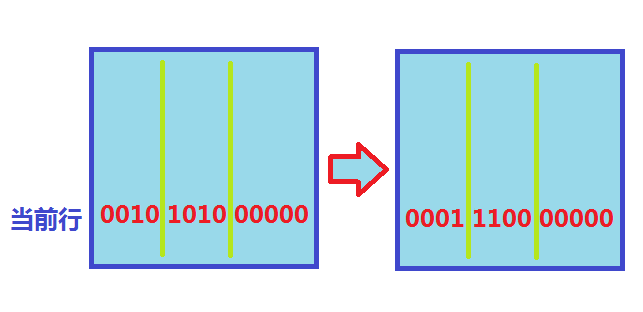
\includegraphics[width=\textwidth]{fig1.png}
				\caption{直接靠拢}
			\end{minipage}
			\begin{minipage}{.45\textwidth}
				\centering
				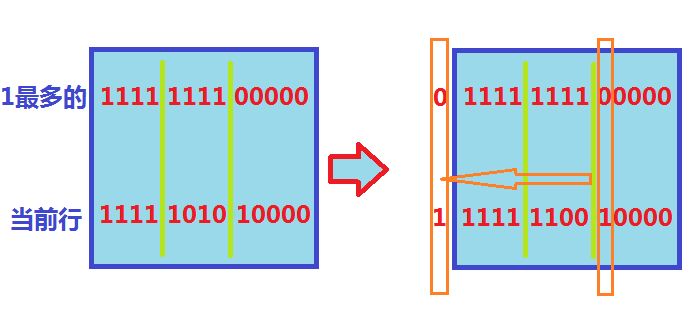
\includegraphics[width=\textwidth]{fig2.png}
				\caption{移动到最前面}
			\end{minipage}
		\end{figure}
		
		我们只能移动最左边和最右边有1的组,而中间的组中假设有0怎么移动也不能变得合法。所以“靠拢”完后,要检查是否使此行所有的1都靠在一起,如果不能就输出“NO”。接着我们把此行即有0又有1的组分离成两个组,一个包含0,一个包含1,我们还要确认最右侧的组是否能维持“特殊”。因为组间是有序的,这样无论以后怎么变换这行都一直会保持合法。为了使这行合法也仅此一种方案,所以如果数据有解这样一定能找到解。
		
		重复找出这样的行并执行“靠拢”,直到所有未确定是否合法的行中的1都仅在一个组中而无法执行“靠拢”。然后在这些组中再找出其中1最多的行分组,重复整个过程,直到所有的行都被标记为合法为止。
		
		记先找1最多的行再重复“靠拢”的过程为P,每次找行要么找到了需要“靠拢”的行,要么找不到而结束这次过程P。因为要操作的行只有n条而过程P只会递归地执行$O(n)$次,所以找行的过程一共要执行$O(n)$次。每次找行要用$O(n)$的时间扫描所有行,每次要用$O(n)$时间找出其所属组并判断是否需要操作“特殊”组,此外每次找到行后还需要使用$O(n^2)$的时间进行列的重组,所以总时间是$O(n^3)$的,空间复杂度$O(n^2)$,期望得分100分。
		
	\myparagraph{算法4}
		
		算法3已经可以通过,但是这种方法用了大量的扫描,这是可以优化的。每次“靠拢”我们需要知道每行的1在哪些组内,一开始先预处理好初始状态,每次要分裂一组时,扫描分出的较小的一组,更新受影响的行。重组列的时候不再直接整列移动,而是记录一个标号建立一个矩阵b的列与矩阵a列的对应关系,重组列的时候操作这个标号。因为是扫描分出的较小一组,分裂时总共要扫描$O(nlog_2n)$列,每次更新$O(n)$行,共$O(n^2log_2n)$。重组操作是$O(n^2)$的。
		
		这种方法总时间降低到了$O(n^2log_2n)$,空间复杂度$O(n^2)$,期望得分100分。但是实现比较复杂,题目不作要求。
		
	\myparagraph{算法5}
	
		简单的数据结构优化只能达到$O(n^2log_2n)$,但是本题还可以做到更快。有一种数据结构——PQ树——可以专门处理这种问题。PQ树是一棵有根多叉树,叶子表示一个排列中的元素,这里叶子就表示列。非叶子结点由两种节点组成:P点和Q点,P点的子节点是可以任意改变顺序的,而Q点的子节点只能是一个固定顺序或者其逆序。这样一棵树的所有可能形态就对应了一个排列族。PQ树支持每次插入一个集合I,调整树的结构使集合I中的元素必须“靠在一起”,这个过程是线性的,而这就是本题要做的操作。
		
		扫描每行,将其所有1的位置作为集合I插入,最后遍历整棵树输出可行解即可。PQ树具体实现较为复杂,在OI竞赛中还没有被推广使用,在此讨论其实现方法就偏离了本题解的中心了,故不作详细叙述。
		
		此方法时间复杂度$O(n^2)$,空间复杂度$O(n^2)$,期望得分100分。
	
\end{document}